\section{What is simulation?}

Astronomy is an observational science.  Unlike in terrestrial physics,
we do not have the luxury of being able to build a model system and do
physical experimentation on it to understand the core physics.  We
have to take what nature gives us.  Simulation enables us to build a
model of a system and allows us to do virtual experiments to
understand how this system reacts to a range of conditions and
assumptions.

It's tempting to think that one can download a simulation code, set a
few parameters, maybe edit some initial conditions, run, and then have
a virtual realization of some astrophysical system that you are
interested in.  Just like that.  In practice, it is not this simple.
All simulation codes make approximations---these start even before one
turns to the computer, simply by making a choice of what equations are
to be solved.  The main approximation that we will follow here, is the
{\em fluid approximation} (see Figure~\ref{fig:intro:fluid_scale}).
We don't want to focus on the motions of the individual atoms, nuclei,
electrons, and photons in our system, so we work on a scale that is
much larger than the mean free path of the system.  This allows us to
describe the bulk properties of a fluid element, which in turn is
small compared to the system of interest.

Within the fluid approximation, additional approximations are made,
both in terms of the physics included and how we represent a continuous
fluid in the finite-memory of a computer (the {\em discretization} process).

Typically, we have a system of PDEs, and we need to
convert the continuous functional form of our system into a discrete
form that can be represented in the finite memory of a computer.  This
introduces yet more approximation.

%V\&V

Blindly trusting the numbers that come out of the code is a recipe
for disaster.  You don't stop being a physicist the moment you execute
the code---your job as a computational scientist is to make sure that
the code is producing reasonable results, by testing it against known
problems and your physical intuition.

Simulations should be used to gain insight and provide a physical
understanding.  Because the systems we solve are so nonlinear, small
changes in the code or the programming environment (compilers,
optimization, etc.)  can produce large differences in the numbers
coming out of the code.  That's not a reason to panic.  As such it is
best not to obsess about precise numbers, but rather the trends our
simulations reveal.  To really understand the limits of your
simulations, you should do parameter and convergence studies.

There is no ``\"uber-code''.  Every algorithm begins with
approximations and has limitations.  
Comparisons between different codes are important and common in our
field (see, for example,
\cite{frenk:1999,dimonte:2004,devalborro:2006}), and build confidence
in the results that we are on the right track.

%
\begin{figure}[t]
\centering
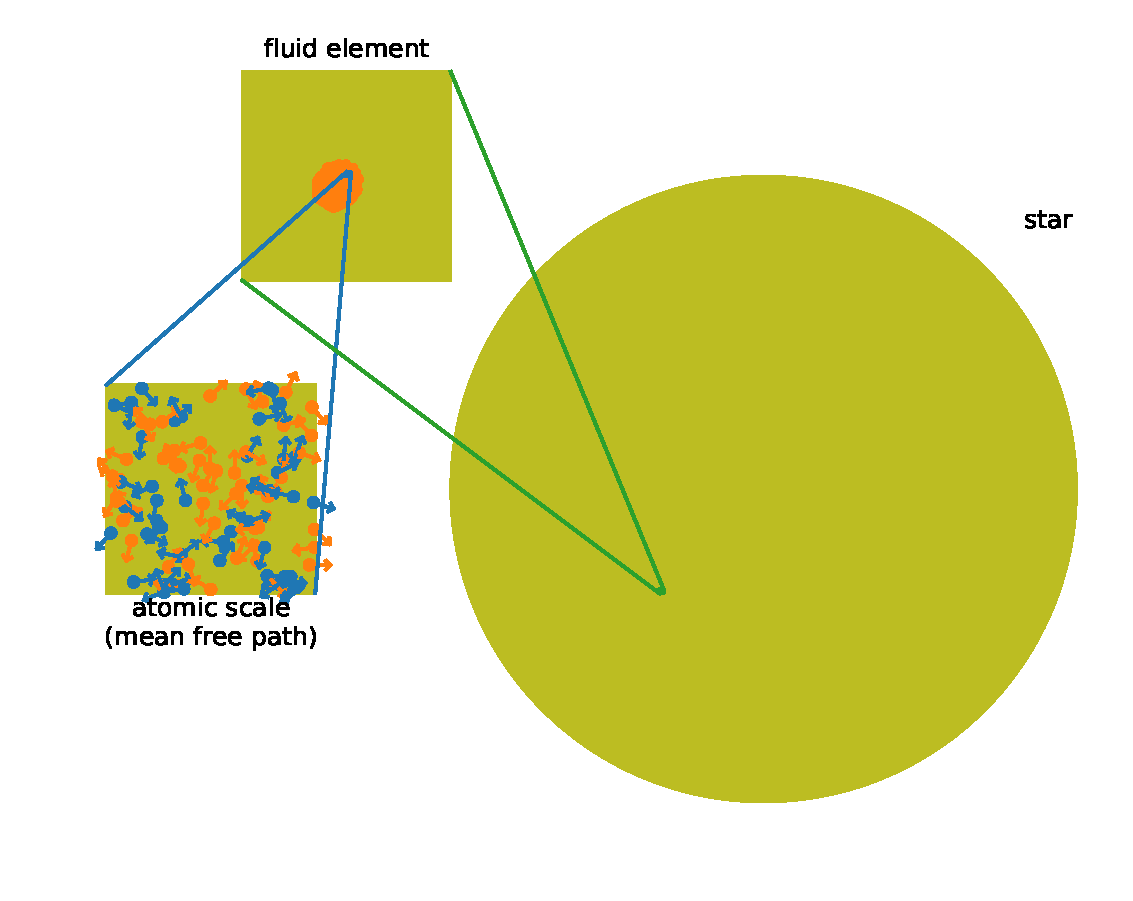
\includegraphics[width=0.9\linewidth]{fluid_scale}
\caption[The fluid scale.]{\label{fig:intro:fluid_scale} The fluid
  scale sits in an intermediate range---much smaller than the system
  of interest (a star in this case), but much larger than the mean
  free path.}
\end{figure}
%

To really understand your simulations, you need to know what the code
your are using is doing under the hood.  This means understanding the
core methods used in our field.  These notes are designed to provide a
basic tour of some of the more popular methods, referring to the key
papers for full derivations and details.  The best way to learn is to
code up these methods for yourself.  A companion python code, {\sf
  pyro} is available to help, and most of the exercises (or
corresponding figures) have links to simple codes that are part of the \hydroex\
repository\footnote{look for the \hydroexsymb\ symbol.}. Descriptions
and links to these codes are found in the appendices.


\section{Numerical basics}

We assume a familiarity with basic numerical methods, which we
summarize below.  Any book on numerical methods can provide a
deeper discussion of these methods.  Some good choices are the
texts by Garcia~\cite{garcia}, Newman~\cite{newman}, and Pang~\cite{pang}.

\subsection{Sources of error}

With any algorithm, there are two sources of error we are concerned
with: {\em roundoff error} and {\em truncation error}.

Roundoff arises from the error inherent in representing a floating
point number with a finite number of bits in the computer memory.  An
excellent introduction to the details of how computers represent
numbers is provided in \cite{goldberg:1991}.

\begin{exercise}[Floating point]
In your choice of programming language, create a floating point
variable and initialize it to 0.1.  Now, print it out in full
precision (you may need to use format specifiers in your language to
get all significant digits the computer tracks).  

You should see that it is not exactly 0.1 to the computer---this is
the floating point error.  The number 0.1 is not exactly representable
in the binary format used for floating point.
\end{exercise}


\begin{exercise}[Machine epsilon]
To see roundoff error in action, write a program to find the value of
$\epsilon$ for which $1 + \epsilon = 1$.  Start with $\epsilon = 1$
and iterate, halving $\epsilon$ each iteration until $1 + \epsilon =
1$. This last value of $\epsilon$ for which this was not true is
the {\em machine epsilon}.  You will get a different value for
single- vs.\ double-precision floating point arithmetic.
\end{exercise}

Some reorganization of algorithms can help minimize roundoff,
e.g.\ avoiding the subtraction of two very large numbers by factoring as:
\begin{equation}
x^3 - y^3 = (x - y)(x^2 + xy + y^2) \enskip ,
\end{equation}
but roundoff error will always be present at some level.

Truncation error is a feature of an algorithm---we typically
approximate an operator or function by expanding about some small
quantity.  When we throw away higher-order terms, we are truncating
our expression, and introducing an error in the representation.  If
the quantity we expand about truly is small, then the error is small.
A simple example is to consider the Taylor series representation of
$\sin(x)$:
\begin{equation}
\sin(x) = \sum_{n=1}^\infty (-1)^{n-1} \frac{x^{2n-1}}{(2n-1)!}
\end{equation}
For $|x| \ll 1$, we can approximate this as:
\begin{equation}
\sin(x) \approx x - \frac{x^3}{6}
\end{equation}
in this case, our truncation error has the leading term $\propto x^5$,
and we say that our approximation is $\mathcal{O}(x^5)$, or
$5^\mathrm{th}$-order accurate.

\begin{exercise}[Convergence and order-of-accuracy]
We will be concerned with the order-of-accuracy of our methods, and a
good way to test whether our method is behaving properly is to perform
a convergence test.  Consider our $5^\mathrm{th}$-order accurate
approximation to $\sin(x)$ above.  Pick a range of $x$'s ($< 1$), and
compute the error in our approximation as
\begin{equation*}
\epsilon \equiv \sin(x) - [  x - x^3/6 ]
\end{equation*}
and show that as you cut $x$ in half, $|\epsilon|$
reduces by $2^5$---demonstrating $5^\mathrm{th}$-order accuracy.
\end{exercise}

This demonstration of measuring the error as we vary the size
of our small parameter is an example of a {\em convergence test}.

\subsection{Differentiation and integration}

For both differentiation and integration, there are two cases we might
encounter:
\begin{enumerate}
\item We have function values, $f_0$, $f_1$, $\ldots$, at a discrete
  number of points, $x_0$, $x_1$, $\ldots$, and we want to compute the
  derivative at a point or integration over a range of points.
\item We know a function analytically and we want to construct a
  derivative or integral of this function numerically. 
\end{enumerate}

 In these notes, we will mainly be concerned with the first case.

\subsubsection{Differentiation of discretely-sampled function}
\label{ch:intro:diff}
Consider a collection of equally spaced points, labeled with an index
$i$, with the physical spacing between them denoted $\Delta
x$.  \MarginPar{show a figure} We can express the first derivative of
a quantity $a$ at $i$ as:
\begin{equation}
\left . \frac{\partial a}{\partial x} \right |_i \approx \frac{a_i - a_{i-1}}{\Delta x}
\end{equation}
or
\begin{equation}
\left . \frac{\partial a}{\partial x} \right |_i \approx \frac{a_{i+1} - a_i}{\Delta x}
\end{equation}
%
(Indeed, as $\Delta x \rightarrow 0$, this is the definition of a
derivative we learned in calculus.)  Both of these are {\em one-sided
  differences}.  By Taylor expanding the data about $x_i$, we see
\begin{equation}
a_{i+1} = a_i + \Delta x \left . \frac{\partial a}{\partial x} \right |_i + \frac{1}{2} \Delta x^2 \left . \frac{\partial^2 a}{\partial x^2} \right |_i + \ldots
\end{equation}
Solving for ${\partial a}/{\partial x} |_i$, we see
\begin{align}
\left . \frac{\partial a}{\partial x} \right |_i &= 
    \frac{a_i - a_{i-1}}{\Delta x} - \frac{1}{2}\Delta x \left . \frac{\partial^2 a}{\partial x^2} \right |_i + \ldots \\ 
%
 &= \frac{a_i - a_{i-1}}{\Delta x} + \mathcal{O}(\Delta x)
\end{align}
where $\mathcal{O}(\Delta x)$ indicates that the leading term in the
error for this approximation is $\sim \Delta x$\footnote{in some
  texts, you see this $\mathcal{O}(\Delta x^n)$ referred to as ``big O
  notation''}.  We say that this is {\em first order accurate}.  This
means that we are neglecting terms that scale as $\Delta x$ or to
higher powers.  This is fine if $\Delta x$ is small.  This error is our
truncation error---just as discussed above, it arises because our
numerical approximation throws away higher order terms.  The
approximation ${\partial a}/{\partial x} |_i = ({a_{i+1} -
  a_i})/{\Delta x}$ has the same order of accuracy.

\begin{exercise}[Truncation error]
{Show that a centered difference,
 \begin{equation*}
\left .\frac{\partial a}{\partial x} \right |_i = \frac{a_{i+1} - a_{i-1}}{2 \Delta x}
\end{equation*}
is second order
accurate, i.e.\ its truncation error is $\mathcal{O}(\Delta x^2)$.}
\end{exercise}

% this figure was created by hydro_examples/basics/derivatives/derivatives.py
\begin{figure}[t]
\centering
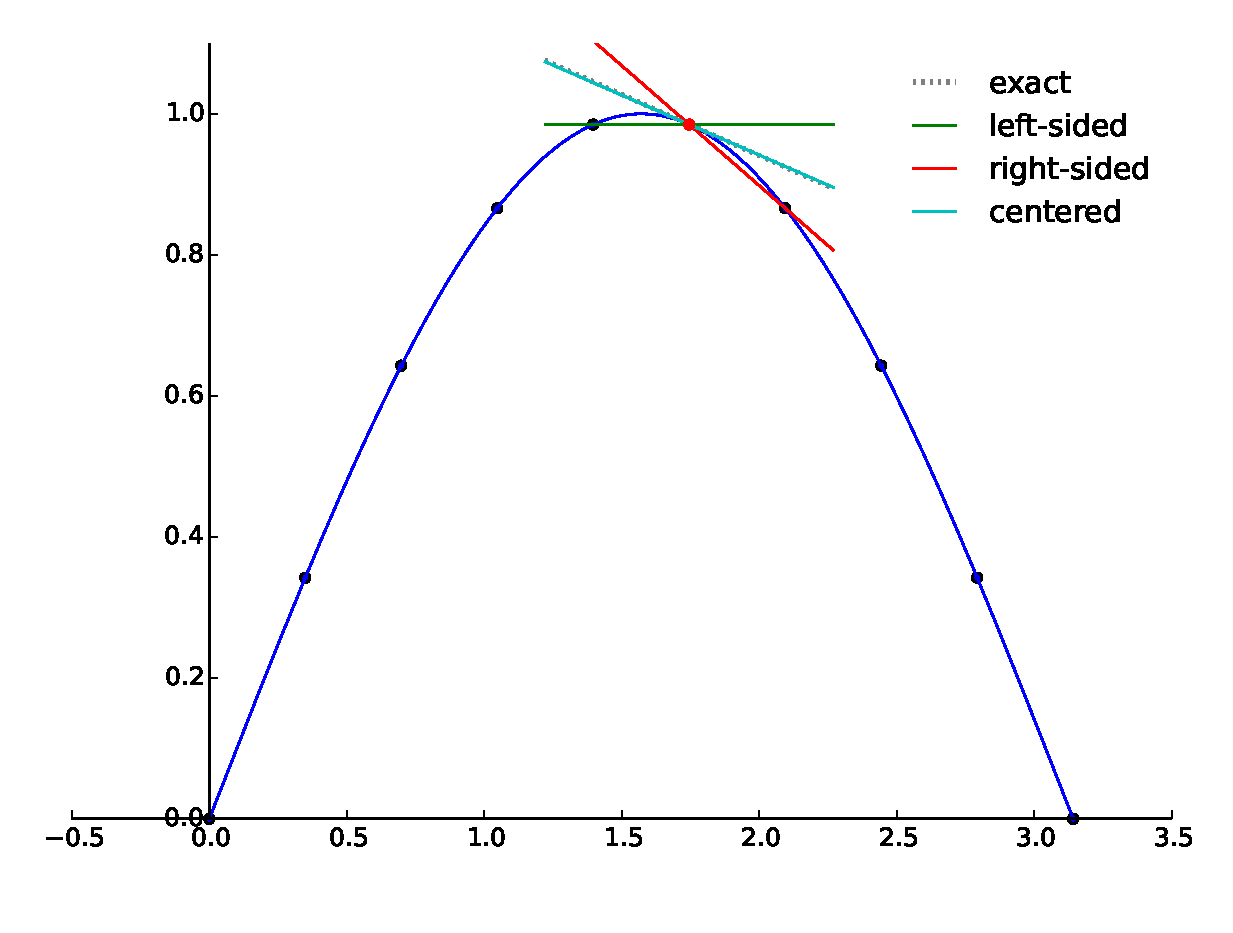
\includegraphics[width=0.8\linewidth]{derivs}
\caption[Difference approximations to the derivative of $\sin(x)$]
        {\label{fig:derivs} A comparison of one-sided and centered
          difference approximations to the derivative of $\sin(x)$.
\hydroexdoit{\href{https://github.com/zingale/hydro_examples/blob/master/basic_numerics/derivatives/derivatives.py}{derivatives.py}}}
\end{figure}

Figure~\ref{fig:derivs} shows the left- and right-sided first-order
differences and the central difference as approximations to
$\sin(x)$. Generally speaking, higher-order methods have lower
numerical error associated with them, and also involve a wider range
of data points.

Second- and higher-order derivatives can be constructed in the same fashion.

\begin{exercise}[Second derivative]
{Using the Taylor expansions for $a_{i+1}$ and $a_{i-1}$, find a difference
approximation to the second derivative at $i$.}
\end{exercise}

\subsubsection{Differentiation of an analytic function}

An alternate scenario is when you know the analytic form of the
function, $f(x)$, and are free to choose the points where you evaluate
it.  Here you can pick a $\delta x$ and evaluate the derivative as
\begin{equation}
\left . \frac{df}{dx} \right |_{x=x_0} =  \frac{f(x_0+\delta x) - f(x_0)}{\delta x}
\end{equation}
An optimal value for $\delta x$ requires a balance of truncation error
(which wants a small $\delta x$) and roundoff error (which becomes
large when $\delta x$ is close to machine $\epsilon$).
Figure~\ref{fig:deriv_error} shows the error for the numerical
derivative of $f(x) = \sin(x)$ at the point $x_0 = 1$, as a function
of $\delta x$.  A nice discussion of this is given in \cite{yak}.  A
good rule-of-thumb is to pick $\delta x \approx \sqrt{\epsilon}$,
where $\epsilon$ is machine epsilon, to balance roundoff and
truncation error.

Comparing the result with different choices of $\delta x$ allows for
error estimation and an improvement of the result by combining the
estimates using $\delta x$ and $\delta x/2$ (this is the basis for a
method called {\em Richardson extrapolation}).

\begin{figure}
  \centering
  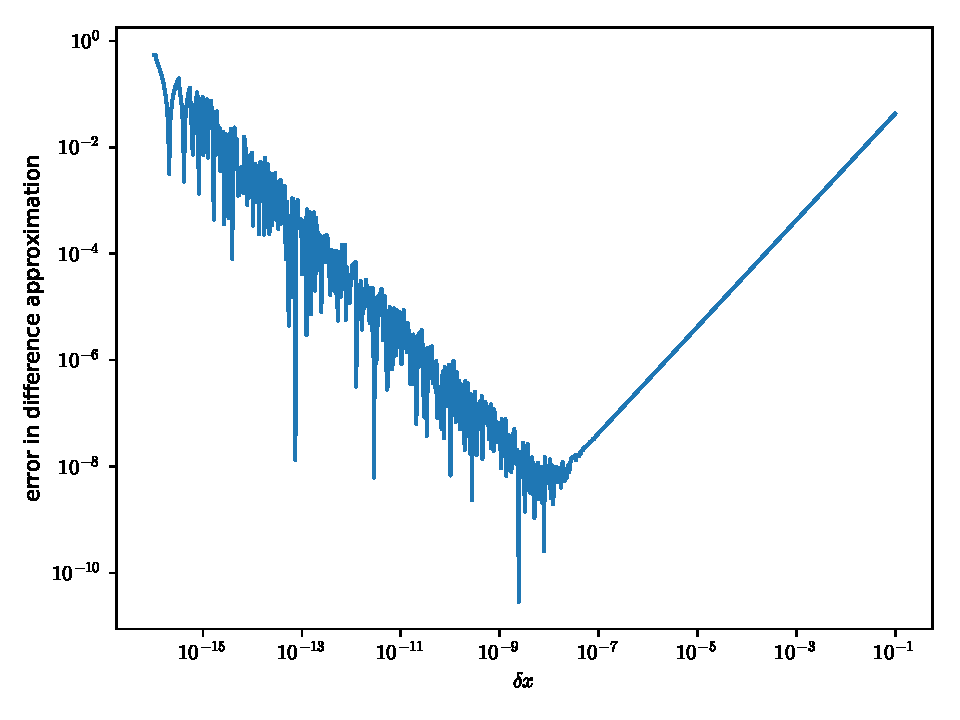
\includegraphics[width=0.8\linewidth]{deriv_error}
  \caption[Error in numerical derivatives] {\label{fig:deriv_error}
    Error in the numerical approximation of the derivative of $f(x) =
    \sin(x)$ at $x_0 = 1$ as a function of the spacing $\delta x$.  For
    small $\delta x$, roundoff error dominates the error in the
    approximation.  For large $\delta x$, truncation error dominates. \\
    \hydroexdoit{\href{https://github.com/zingale/hydro_examples/blob/master/basic_numerics/derivatives/deriv_error.py}{deriv\_error.py}}}
\end{figure}




\subsubsection{Integration}

In numerical analysis, any integration method that is composed as a
weighted sum of the function evaluated at discrete points is called a
{\em quadrature rule}.

If we have a function sampled at a number of
equally-spaced points, $x_0 \equiv a, x_1, \ldots, x_N \equiv
b$\footnote{Note that this is $N$ intervals and $N+1$ points}, we can
construct a discrete approximation to an integral as:
\begin{equation}
I \equiv \int_a^b f(x) dx \approx \Delta x \sum_{i = 0}^{N-1} f(x_i)
\end{equation}
where $\Delta x \equiv (b-a)/N$ is the width of the intervals (see the
top-left panel in Figure~\ref{fig:integration}).  This is a very crude
method, but in the limit that $\Delta x \rightarrow 0$ (or $N
\rightarrow \infty$), this will converge to the true integral.  This
method is called the {\em rectangle rule}.  Note that here we
expressing the integral over the $N$ intervals using a simple
quadrature rule in each interval.  Summing together the results of the
integral over each interval to get the result in our domain is called
{\em compound} integration.

We can get a more accurate answer for $I$ by interpolating between the
points.  The simplest case is to connect the sampled function values,
$f(x_0), f(x_1), \ldots, f(x_N)$ with a line, creating a trapezoid in
each interval, and then simply add up the area of all of the
trapezoids:
\begin{equation}
I \equiv \int_a^b f(x) dx \approx
  \Delta x \sum_{i = 0}^{N-1} \frac{f(x_i) + f(x_{i+1})}{2}
\end{equation}
This is called the {\em trapezoid rule} (see the top-right panel in
Figure~\ref{fig:integration}).  Note here we assume that the points
are equally spaced.

One can keep going, but practically speaking, a quadratic interpolation
is as high as one usually encounters.  Fitting a quadratic polynomial
requires three points.

\begin{exercise}[Simpson's rule for integration]
\label{ex:simpsons}
Consider a function, $f(x)$, sampled at three equally-spaced points,
$\alpha, \beta, \gamma$, with corresponding function values $f_\alpha,
f_\beta, f_\gamma$.  Derive the expression for Simpson's rule by
fitting a quadratic $\hat{f}(x) = A(x - \alpha)^2 + B(x - \alpha) + C$
to the three points (this gives you $A$, $B$, and $C$), and then
analytically integrating $\hat{f}(x)$ in the interval
$[\alpha,\gamma]$.  You should find
\begin{equation}
I = \frac{\gamma-\alpha}{6} (f_\alpha + 4f_\beta + f_\gamma)
\end{equation}
Note that $(\gamma-\alpha)/6 = \Delta x/3$
\end{exercise}

For a number of samples, $N$, in $[a,b]$, we will
consider every two intervals together.  The resulting expression is:
\begin{align}
I &\equiv \int_a^b f(x) dx
\approx  \frac{\Delta x}{3} \sum_{i = 0}^{(N-2)/2} \left [f(x_{2i}) + 4 f(x_{2i+1}) + f(x_{2i+2}) \right ] \\
&= f(x_0) + 4f(x_1) + 2f(x_2) + 4f(x_3) + 2f(x_4) + \ldots + \nonumber 2f(x_{N-2}) + 4f(x_{N-1}) + f(x_N)
\end{align}
This method is called {\em Simpson's rule}.  Note that for 2 intervals
/ 3 sample points ($N=2$), we only have 1 term in the sum, $(N-2)/2 =
0$, and we get the result derived in Exercise~\ref{ex:simpsons}.


Figure~\ref{fig:integration} shows
these different approximations for the case of two intervals (three points).

% these figures were created with figures/intro/integrals.py
\begin{figure}
\centering
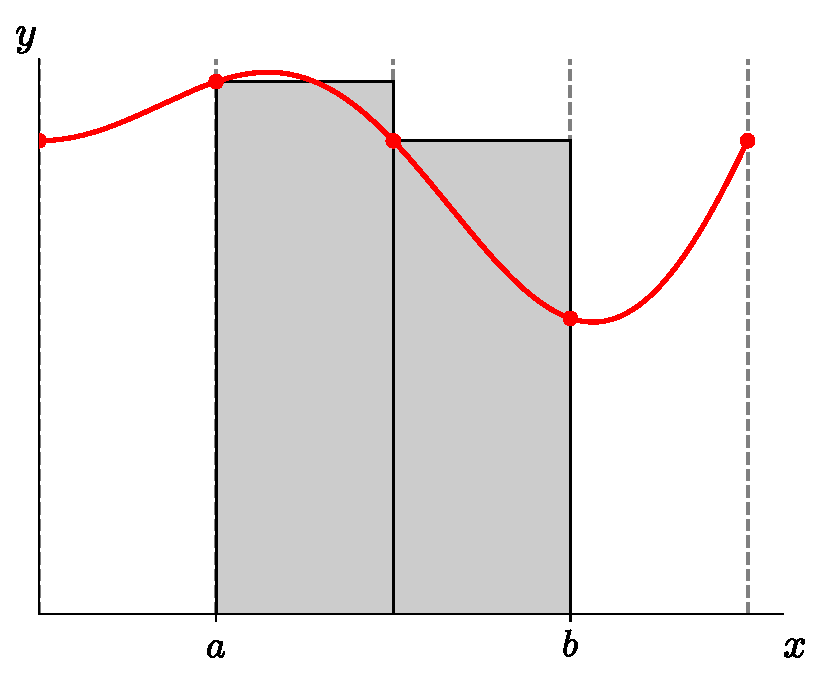
\includegraphics[width=0.49\linewidth]{rectangle}
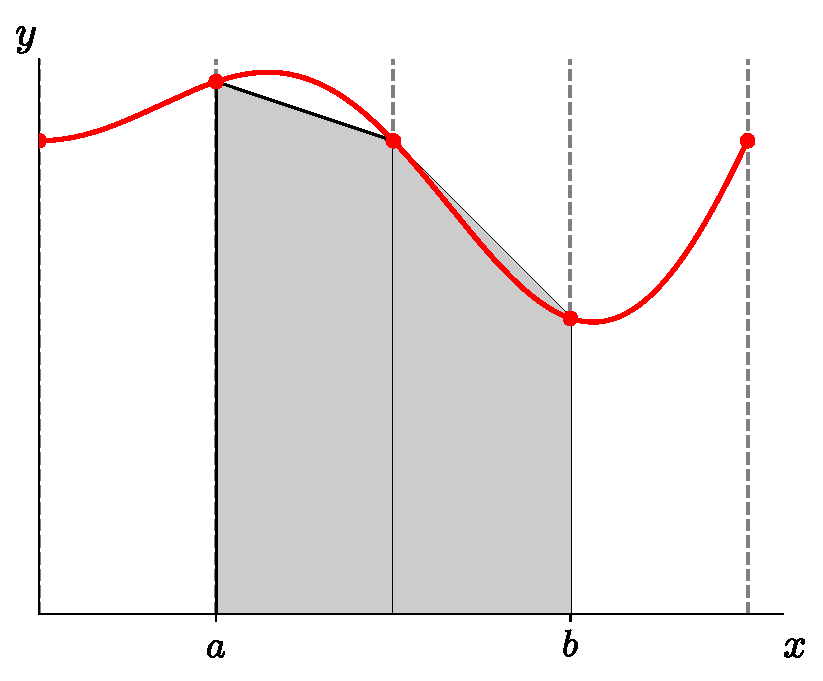
\includegraphics[width=0.49\linewidth]{trapezoid} \\
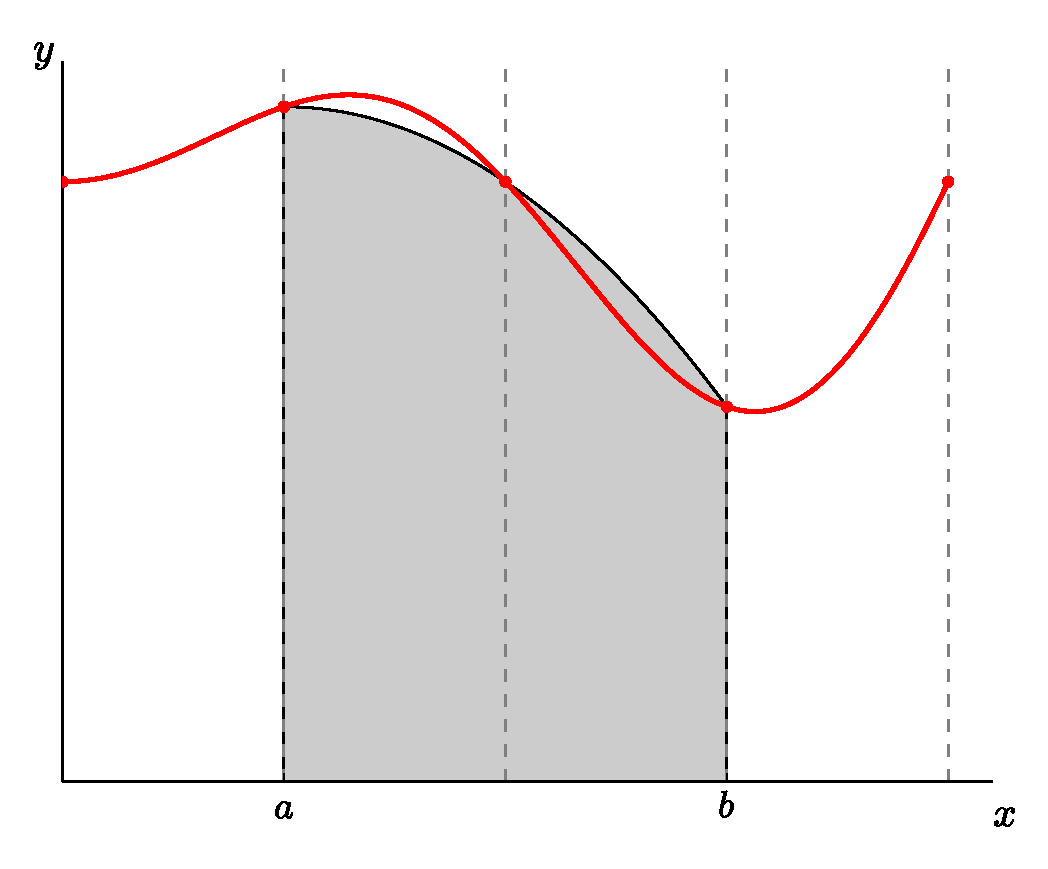
\includegraphics[width=0.49\linewidth]{simpsons}
\begin{minipage}[b]{0.49\linewidth}
\caption[Integration rules]{\label{fig:integration} The rectangle rule
  (top left), trapezoid rule (top right) and Simpson's rule (left) for
  integration.}
\end{minipage}
\end{figure}


Analogous expressions exist for the case of unequally-spaced points.

The compound trapezoid rule converges as second-order over the
interval $[a,b]$, while Simpson's rule converges as fourth-order.

As with differentiation, if you are free to pick the points where you
evaluate $f(x)$, you can get a much higher-order accurate result.
{\em Gaussian quadrature} is a very powerful technique that uses the
zeros of different polynomials as the evaluation points for the
function to give extremely accurate results.  See the text by
Garcia~\cite{garcia} for a nice introduction to these methods.


\subsection{Root finding}

Often we want to find the root of a function (or the vector that zeros
a vector of functions).  The most popular method for root finding is
the {\em Newton-Raphson method}.  We want to find $x$, such that $f(x)
= 0$.  Start with an initial guess $x_0$ that you believe is close to
the root, then you can improve the guess to the root by an amount
$\delta x$ by looking at the Taylor expansion about $x_0$:
\begin{equation}
f(x_0 + \delta x) \sim f(x_0) + f^\prime(x_0) \delta x + \ldots = 0
\end{equation}
Keeping only to $\mathcal{O}(\delta x)$, we can solve for the correction, $\delta x$:
\begin{equation}
\label{eq:intro:newtonsmethod}
  \delta x = -\frac{f(x_0)}{f^\prime(x_0)}
\end{equation}
This can be used to correct out guess as $x_0 \leftarrow x_0 + \delta
x$, and we can iterate on this procedure until $\delta x$ falls below
some tolerance.  Figure~\ref{fig:newtonsmethod} illustrates this
iteration.

\begin{figure}
\centering
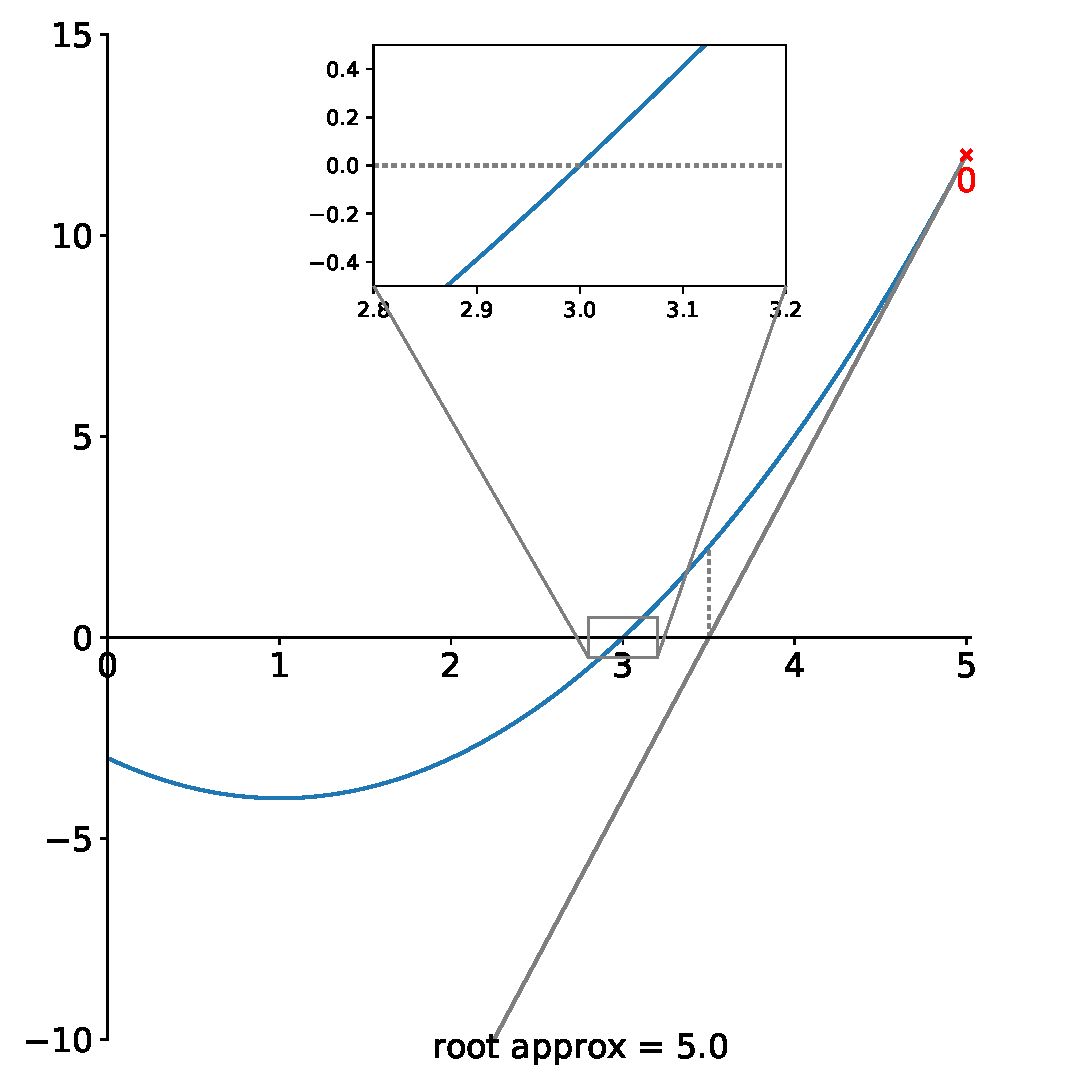
\includegraphics[width=0.49\linewidth]{newton_00}
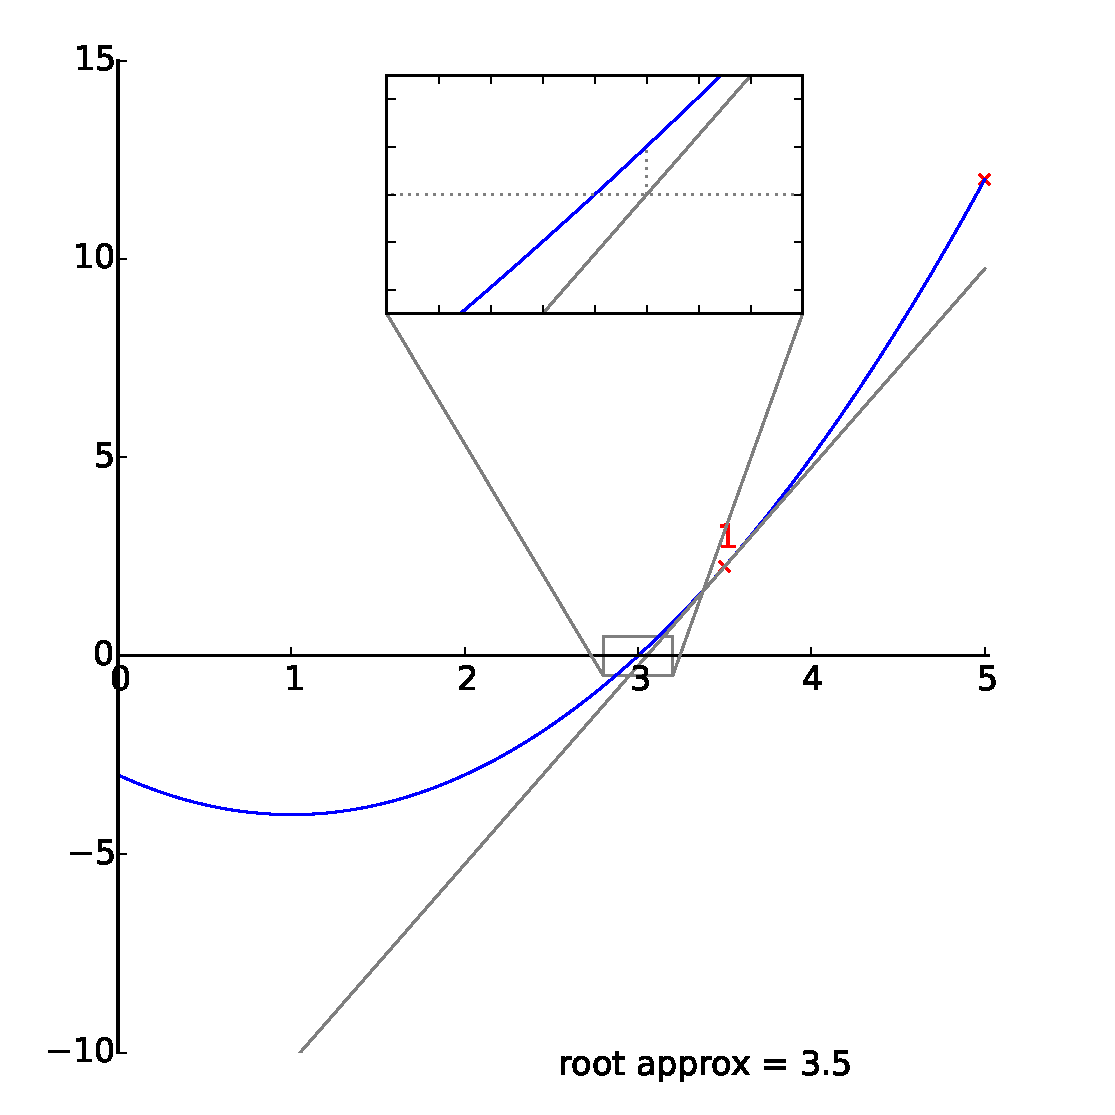
\includegraphics[width=0.49\linewidth]{newton_01} \\[1em]
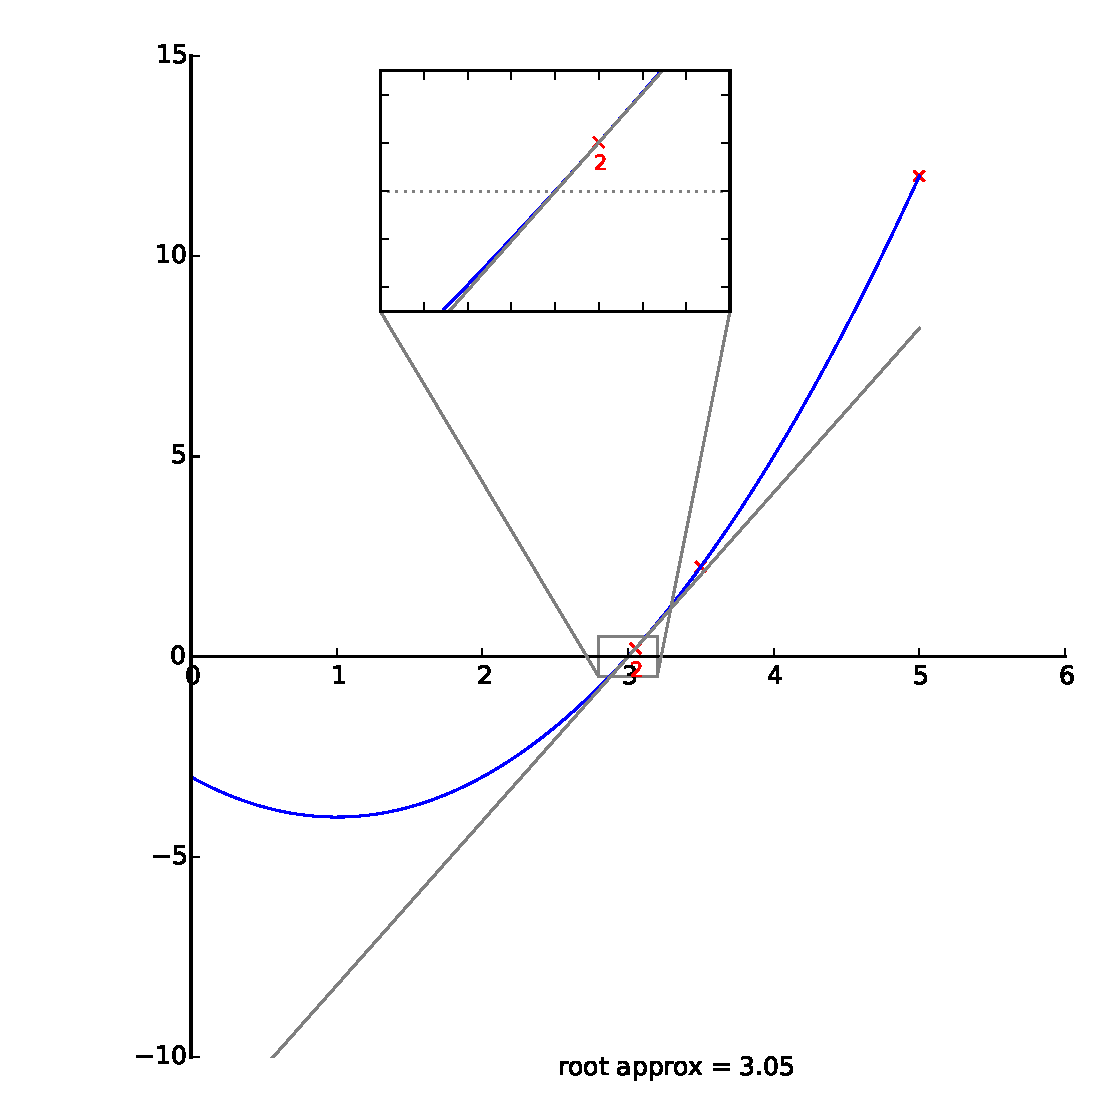
\includegraphics[width=0.49\linewidth]{newton_02}
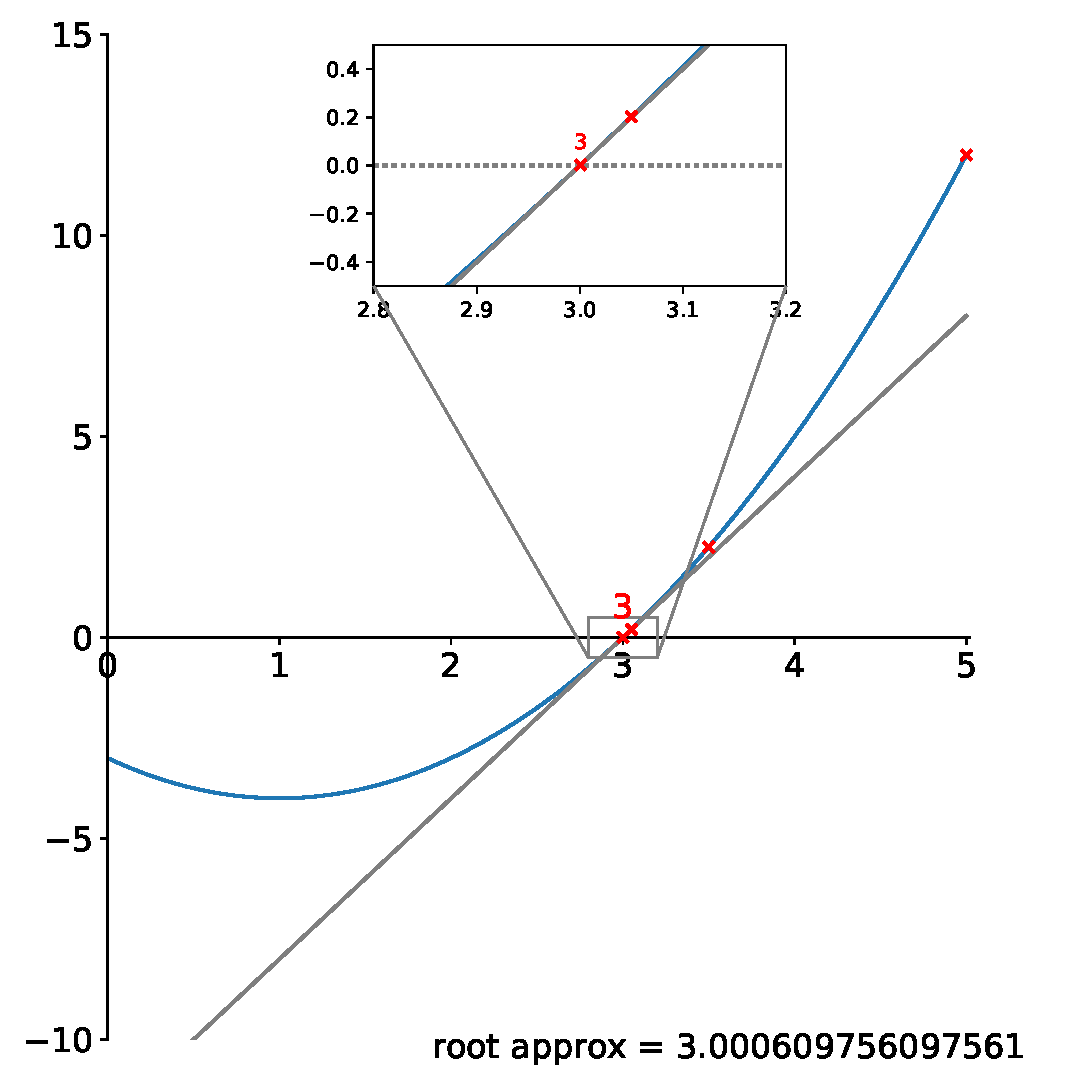
\includegraphics[width=0.49\linewidth]{newton_03}
\caption[Convergence of Newton's method for root
  finding]{\label{fig:newtonsmethod} The convergence of Newton's
  method for finding the root.  In each pane, the red point is the
  current guess for the root.  The solid gray line is the
  extrapolation of the slope at the guess to the $x$-axis, which
  defines the next approximation to the root.  The vertical dotted
  line to the function shows the new slope that will be used for
  extrapolation in the next iteration. \\
\hydroexdoit{\href{https://github.com/zingale/hydro_examples/blob/master/basic_numerics/roots/roots_plot.py}{roots\_plot.py}}}
\end{figure}


The main ``got-ya'' with this technique is that you need a good initial
guess.  In the Taylor expansion, we threw away the $\delta x^2$ term,
but if our guess was far from the root, this (and higher-orders) term
may not be small.  Obviously, the derivative must be non-zero in the
region around the root that you search as well.

\begin{exercise}[Newton's method]
{Code up Newton's method for finding the root of a function $f(x)$
and test it on several different test functions.}
\end{exercise}
The {\em secant method} for root finding is essentially
Newton-Raphson, but instead of using an analytic derivative,
$f^\prime$ is estimated as a numerical difference.

Newton's method has pathologies---it is possible to get into a cycle
where you don't converge but simply pass through the same set of root
approximations.  Many other root finding methods exist, including {\em
  bisection}, which iteratively halves an interval known to contain a
root by looking for the change in sign of the function $f(x)$.  {\em
  Brent's method} combines several different methods to produce a
robust procedure for root-finding.  Most numerical analysis texts will
give a description of these.

\subsection{Norms}

\label{intro:sec:norm}

Often we will need to measure the ``size'' of an error to a discrete
approximation.  For example, imagine that we know the exact function,
$f(x)$ and we have have an approximation, $f_i$ defined at $N$ points,
$i = 0, \ldots, N-1$.  The error at each point $i$ is $\epsilon_i =
|f_i - f(x_i)|$.  But this is $N$ separate errors---we want a single
number that represents the error of our approximation.  This is the
job of a vector norm.  

There are many different norms we can define.  For a vector ${\bf q}$,
we write the norm as $\|q\|$.  Often, we'll put a subscript after the
norm brackets to indicate which norm was used.  Some popular norms
are:
\begin{itemize}
\item {\em inf norm}: 
  \begin{equation} 
    \| q \|_\infty = \max_i |q_i|
  \end{equation}

\item {\em L1 norm}:
  \begin{equation}
    \| q \|_1 = \frac{1}{N} \sum_{i=0}^{N-1} |q_i|
  \end{equation}

\item {\em L2 norm}:
  \begin{equation}
    \| q \|_2 = \left [ \frac{1}{N} \sum_{i=0}^{N-1} |q_i|^2 \right ]^{1/2}
  \end{equation}

\item {\em general p-norm}
  \begin{equation}
    \| q \|_p = \left [ \frac{1}{N} \sum_{i=0}^{N-1} |q_i|^p \right ]^{1/p}
  \end{equation}

\end{itemize}

Note that these norms are defined such that they are normalized---if
you double the number of elements ($N$), the normalization gives you a
number that can still be meaningfully compared to the smaller set.
For this reason, we will use these norms when we look at the
convergence with resolution of our numerical methods.

We'll look into how the choice of norm influences you convergence
criterion, but inspection shows that the inf-norm is local---a element
in your vector is given the entire weight, whereas the other norms are
more global.

\subsection{ODEs}

Consider a system of first-order ordinary differential equations,
\begin{equation}
\dot{\bf y} = {\bf f}(t, {\bf y}(t))
\end{equation}
If $k$ represents an index into the vector ${\bf y}$, then the
$k^\mathrm{th}$ ODE is
\begin{equation}
\dot{y}_k = f_k(t, {\bf y}(t))
\end{equation}
We want to solve for the vector ${\bf y}$ as a function of time.  Note
higher-order ODEs can always be written as a system of first-order
ODEs by introducing new variables\footnote{As an example, consider
  Newton's second law, $\ddot{x} = F/m$.  We can write this as a system
  of two ODEs by introducing the velocity, $v$, giving us: $\dot{v} =
  F/m$, $\dot{x} = v$.}.

Broadly speaking, methods for integrating ODEs can be broken down into
explicit and implicit methods.  Explicit methods difference the system
to form an update that uses only the current (and perhaps previous)
values of the dependent variables in evaluating $f$.  For example, a
first-order explicit update ({\em Euler's method}) appears as:
\begin{equation}
y^{n+1}_k = y^n_k + \Delta t f_k(t^n, {\bf y}^n)
\end{equation}
where $\Delta t$ is the stepsize.  Implicit methods instead evaluate
the righthand side, ${\bf f}$ using the new-time value of ${\bf y}$
we are solving for.

Perhaps the most popular explicit method for ODEs is the 4th-order
Runge-Kutta method (RK4).  This is a multistage method where several
extrapolations to the midpoint and endpoint of the interval are
made to estimate slopes and then a weighted average of these slopes
are used to advance the solution.  The various slopes
are illustrated in Figure~\ref{fig:rk} and the overall procedure looks like:
\begin{equation}
y_k^{n+1} = y_k^n + \frac{\Delta t}{6} (k_1 + 2 k_2 + 2 k_3 + k_4)
\end{equation}
where the slopes are:
\begin{align}
k_1 &= f(t^n, y_k^n) \\
k_2 &= f(t^n + \tfrac{\Delta t}{2}, y_k^n + \tfrac{\Delta t}{2} k_1) \\
k_3 &= f(t^n + \tfrac{\Delta t}{2}, y_k^n + \tfrac{\Delta t}{2} k_2) \\
k_4 &= f(t^n + \Delta t, y_k^n + \Delta t k_3)
\end{align}
Note the similarity to Simpson's method for integration.  This is
fourth-order accurate overall.

\afterpage{\clearpage}
% rk4_plot.py creates rk4_k[1-4].pdf, rk4_final.pdf
\begin{figure}[p]
\centering
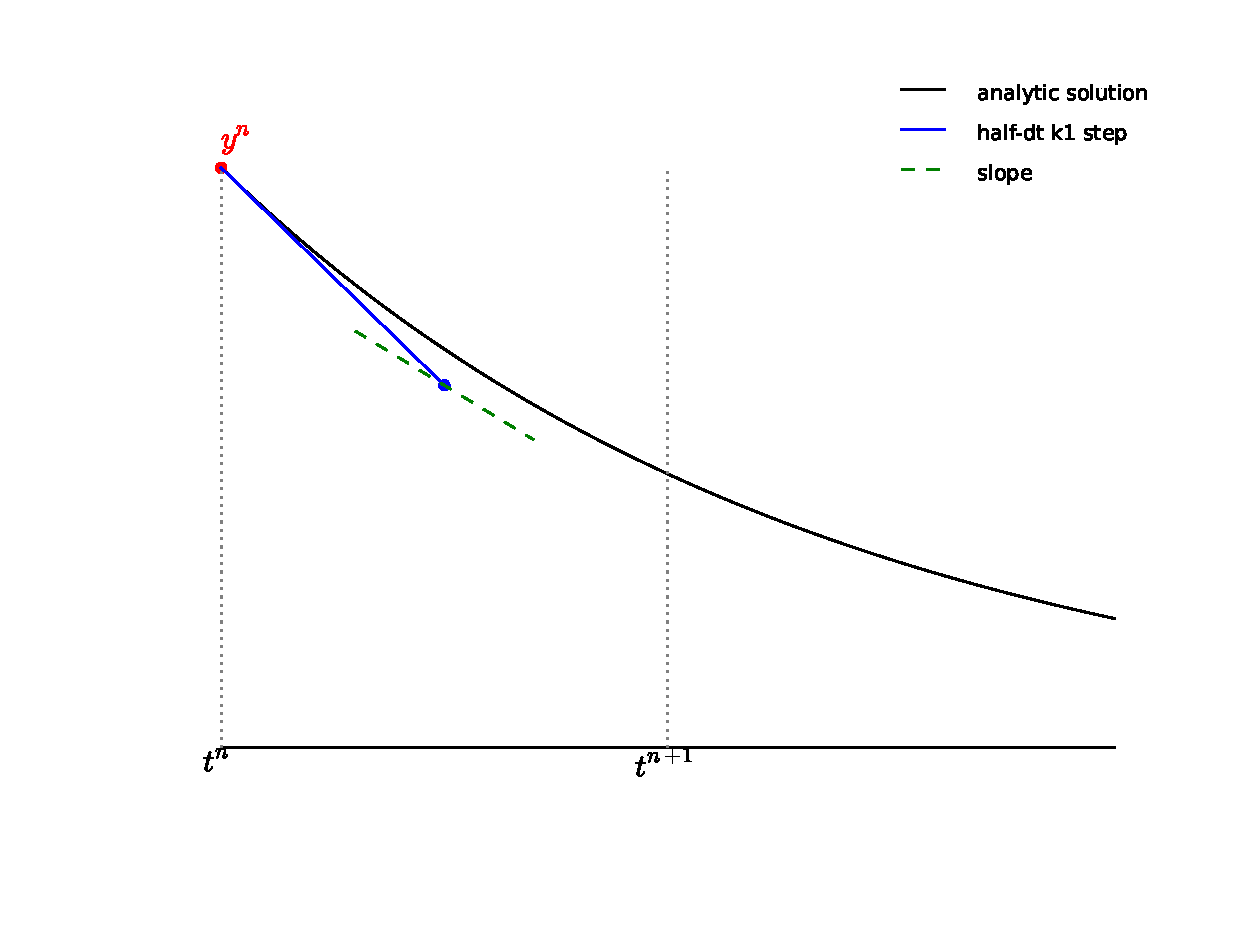
\includegraphics[width=0.48\linewidth]{rk4_k1} 
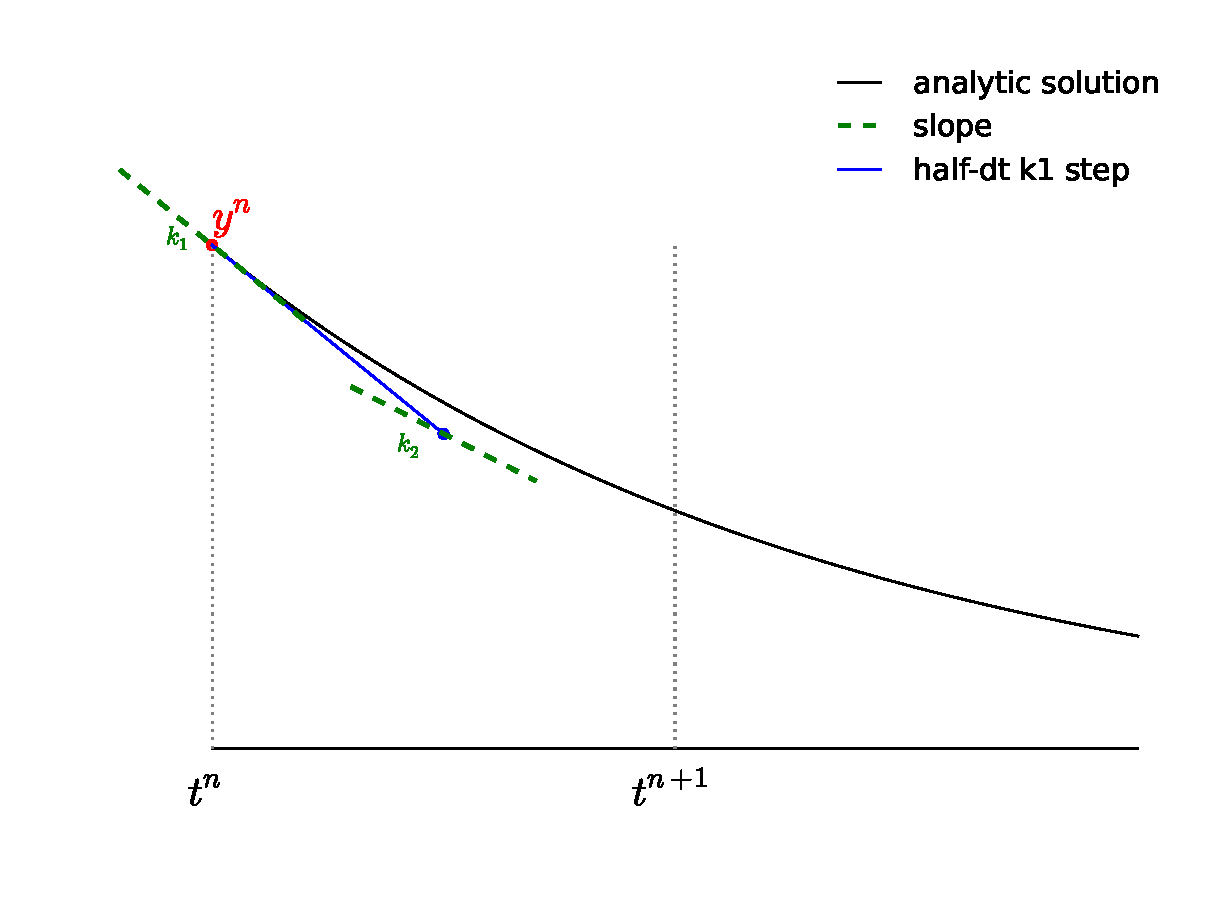
\includegraphics[width=0.48\linewidth]{rk4_k2} \\
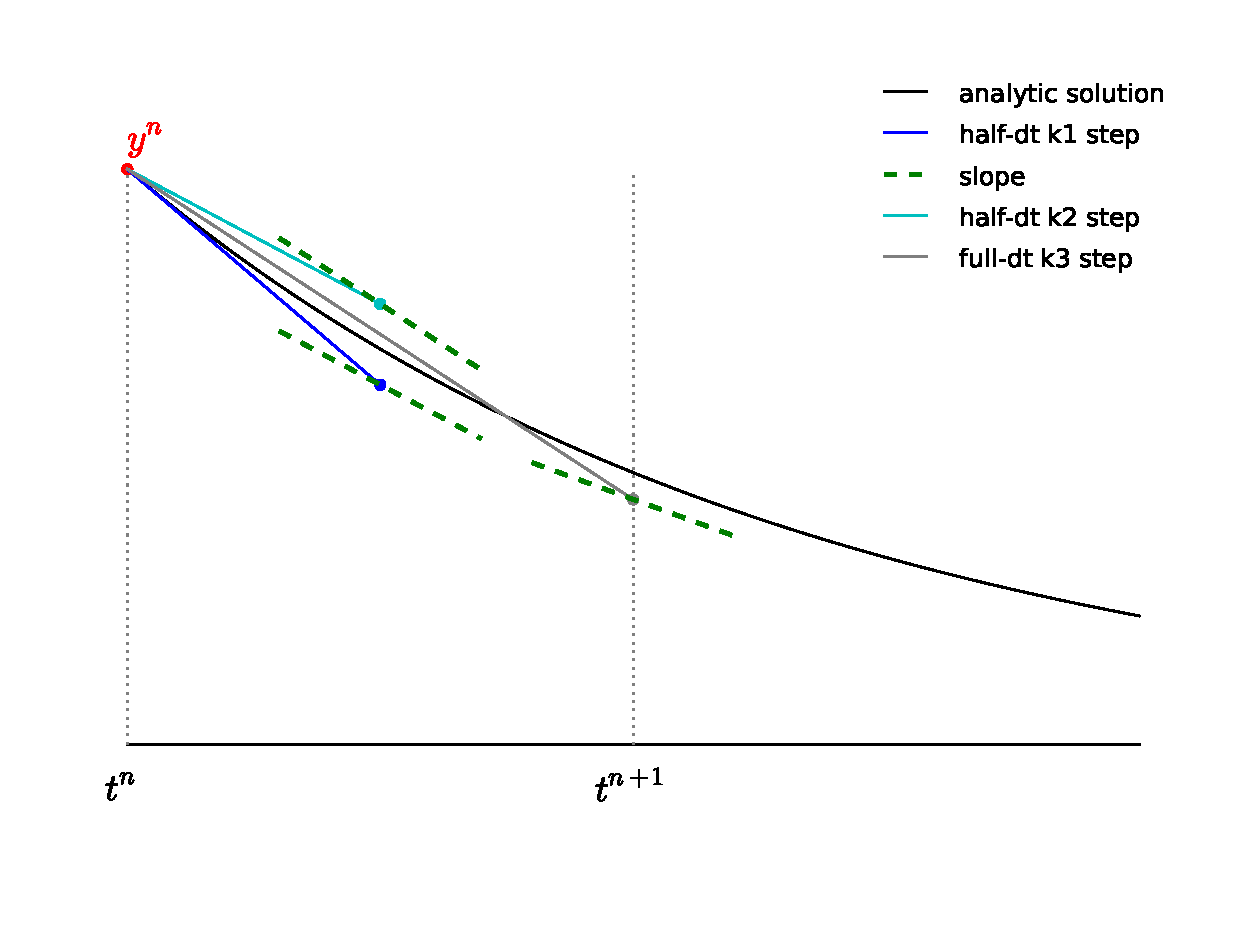
\includegraphics[width=0.48\linewidth]{rk4_k3} 
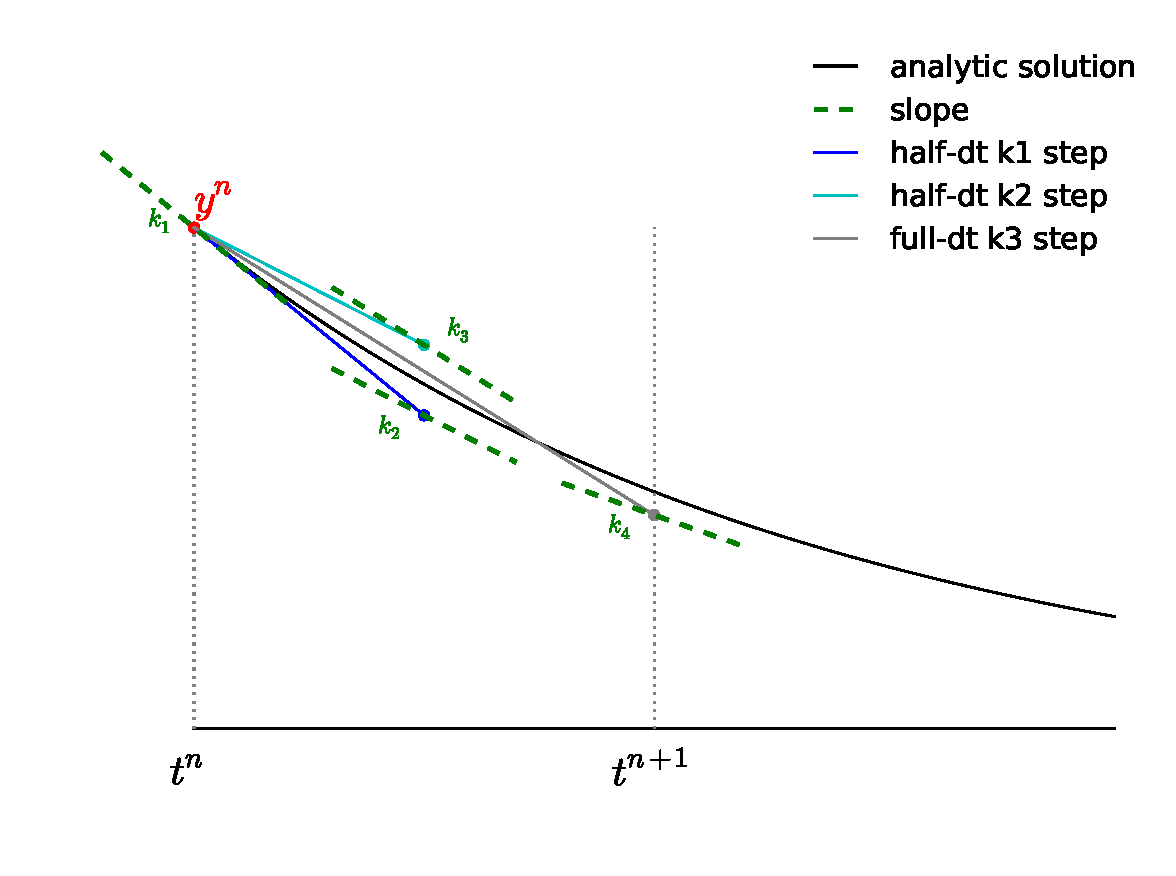
\includegraphics[width=0.48\linewidth]{rk4_k4} \\
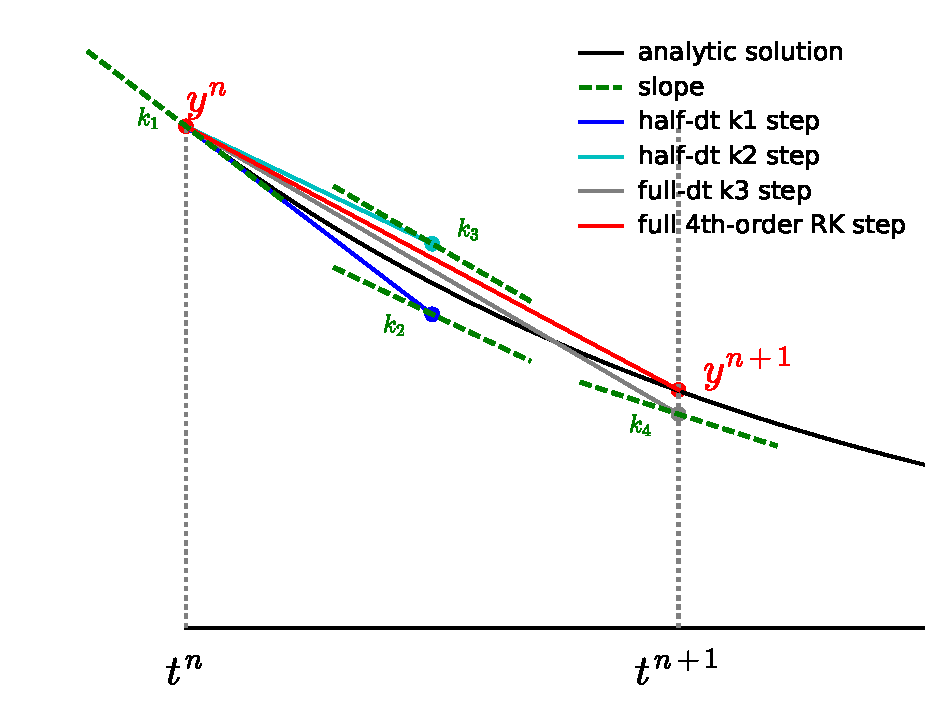
\includegraphics[width=0.6\linewidth]{rk4_final}
%
\caption[The $4^\mathrm{th}$-order Runge-Kutta method] {\label{fig:rk}
  A graphical illustration of the four steps in the
  $4^\mathrm{th}$-order Runge-Kutta method.  This example
  is integrating $dy/dt = -y$.}
\end{figure}


\begin{exercise}[ODE accuracy]
Consider the orbit of Earth around the Sun.  If we work in the units
of astronomical units, years, and solar masses, then Newton's gravitational
constant and the solar mass together are simply $G M = 4\pi^2$ (this
should look familiar as Kepler's third law).  We
can write the ODE system describing the motion of Earth as:
\begin{align}
\dot{\bf x} &= {\bf v} \\
\dot{\bf v} &= -\frac{G M {\bf r}}{r^3}
\end{align}
If we take the coordinate system such that the Sun is at the origin,
then, ${\bf x} = (x, y)^\intercal$ is the position of the Earth
and ${\bf r} = x {\bf \hat{x}} + y {\bf \hat{y}}$ is the radius
vector pointing from the Sun to the Earth.

Take as initial conditions the planet at perihelion:
\begin{align*}
x_0 &= 0 \\
y_0 &= a (1-e) \\
({\bf v}\cdot {\bf \hat{x}})_0 &= -\sqrt{\frac{GM}{a} \frac{1+e}{1-e}} \\
({\bf v}\cdot {\bf \hat{y}})_0 &= 0
\end{align*}
where $a$ is the semi-major axis and $e$ is the eccentricity of the orbit
(these expressions can be found in any introductory astronomy text that
discusses Kepler's laws).

Integrate this system for a single orbital period with the first-order
Euler and the RK4 method and measure the convergence by integrating at
a number of different $\Delta t$'s.  Note: you'll need to define some
measure of error, you can consider a number of different metrics, e.g.,
the change in radius after a single orbit.
\end{exercise}
\MarginPar{show figure}

The choice of the stepsize, $\Delta t$, in the method greatly affects
the accuracy.  In practice you want to balance the desire for accuracy
with the expense of taking lots of small steps.  A powerful technique
for doing this is to use error estimation and an adaptive stepsize with
your ODE integrator.  This monitors the size of the truncation error
and adjusts the stepsize, as needed, to achieve a desired accuracy.  A
nice introduction to how this works for RK4 is given in \cite{garcia}.

\subsubsection{Implicit methods}

Implicit methods difference the system in a way that includes the new
value of the dependent variables in the evaluation of $f_k(t,{\bf
  y}(t))$---the resulting implicit system is usually solved using, for
example, Newton-Raphson iteration.

A first-order implicit update
(called {\em backward Euler}) is:
\begin{equation}
  \label{eq:backwardeuler}
{\bf y}^{n+1} = {\bf y}^n + \Delta t {\bf f}(t^{n+1}, {\bf y}^{n+1})
\end{equation}
This is more complicated to solve than the explicit methods above, and
generally will require some linear algebra.  If we take $\Delta t$ to
be small, then the change in the solution, $\Delta {\bf y}$ will be
small as well, and we can Taylor-expand the system.

To solve this, we pick a guess, ${\bf y}^{n+1}_0$, that we think is
close, to the solution and we will solve for a correction, $\Delta
{\bf y}_0$ such that
\begin{equation}
\label{eq:impl_correction}
  {\bf y}^{n+1} = {\bf y}^{n+1}_0 + \Delta {\bf y}_0
\end{equation}
Using this approximation, we can expand the righthand side vector,
\begin{equation}
\label{eq:impl_rhs_expansion}
{\bf f}(t^{n+1},{\bf y}^{n+1}) = {\bf f}(t^{n+1}, {\bf y}^{n+1}_0) +
     \left . \frac{\partial {\bf f}}{\partial {\bf y}} \right |_0 \Delta {\bf y}_0 + \ldots
\end{equation}
Here we recognize the Jacobin matrix, ${\bf J} \equiv \partial {\bf
  f}/\partial {\bf y}$,
\begin{equation}
\renewcommand\arraystretch{1.5}
{\bf J} = \left (
\begin{array}{ccccc}
\partial f_1/\partial y_1 & \partial f_1/\partial y_2 &
\partial f_1/\partial y_3 & \ldots & \partial f_1/\partial y_n \\
%
\partial f_2/\partial y_1 & \partial f_2/\partial y_2 &
\partial f_2/\partial y_3 & \ldots & \partial f_2/\partial y_n \\
%
\vdots  & \vdots & \vdots & \ddots & \vdots \\
%
\partial f_n/\partial y_1 & \partial f_n/\partial y_2 &
\partial f_n/\partial y_3 & \ldots & \partial f_n/\partial y_n \\
\end{array}
\right )
\end{equation}
%
Putting Eqs.~\ref{eq:impl_correction} and \ref{eq:impl_rhs_expansion}
into Eq.~\ref{eq:backwardeuler}, we have:
\begin{equation}
{\bf y}^{n+1}_0 + \Delta {\bf y}_0 = {\bf y}^n + \Delta t \left [
  {\bf f}(t^{n+1}, {\bf y}^{n+1}_0) +
     \left .{\bf J}\right |_0\, \Delta {\bf y}_0 \right ]
\end{equation}
Writing this as a system for the unknown correction, $\Delta {\bf
  y}_0$, we have
\begin{equation}
  \left ({\bf I} - \Delta t \left . {\bf J} \right |_0 \right ) \Delta {\bf y}_0 =
   {\bf y}^n - {\bf y}_0^{n+1} + \Delta t {\bf f}(t^{n+1}, {\bf y}^{n+1}_0)
\end{equation}
This is a linear system (a matrix $\times$ vector $=$ vector) that can
be solved using standard matrix techniques (numerical methods for
linear algebra can be found in most numerical analysis texts).  After
solving, we can correct our initial guess:
\begin{equation}
  {\bf y}^{n+1}_1 = {\bf y}^{n+1}_0 + \Delta {\bf y}_0
\end{equation}

Written this way, we see that we can iterate.  To kick things off, we
need a suitable guess---an obvious choice is ${\bf y}^{n+1}_0 = {\bf
  y}^n$.  Then we correct this guess by iterating, with the $k$-th
iteration looking like:
\begin{align}
  \left ({\bf I} - \Delta t \left . {\bf J} \right |_{k-1} \right ) \Delta {\bf y}_{k-1} &=
        {\bf y}^n - {\bf y}_{k-1}^{n+1} + \Delta t {\bf f}(t^{n+1}, {\bf y}^{n+1}_{k-1}) \\
  {\bf y}^{n+1}_k &= {\bf y}^{n+1}_{k-1} + \Delta {\bf y}_{k-1}
\end{align}
We will iterate until we find $\| \Delta {\bf y}_k\| < \epsilon \|
{\bf y}^n \|$.  Here $\epsilon$ is a small tolerance, and we use ${\bf
  y}^n$ to produce a reference scale for meaningful comparison.  Note
that here we use a vector norm to give a single number for comparison.

Note that the role of the Jacobian here is the same as the first
derivative in the scalar Newton's method for root finding
(Eq.~\ref{eq:intro:newtonsmethod})---it points from the current guess
to the solution.  Sometimes an approximation to the Jacobian, which is
cheaper to evaluate, may work well enough for the method to converge.

Explicit methods are easier to program and run faster (for a given $
\Delta t$), but implicit methods work better for {\em stiff}
problems---those characterized by widely disparate timescales over
which the solution changes~\cite{byrnehindmarsh}\footnote{Defining
  whether a problem is stiff can be tricky (see \cite{byrnehindmarsh}
  for some definitions).  For a system of ODEs, a large range in the
  eigenvalues of the Jacobian usually means it is stiff.}.  A good
example of this issue in astrophysical problems is with nuclear
reaction networks (see, e.g., \cite{timmes_networks}).  As with the
explicit case, higher-order methods exist that can provide better
accuracy at reduced cost.



\subsection{FFTs}

\label{sec:intro:ffts}

The discrete Fourier transform converts a discretely-sampled function
from real space to frequency space, and identifies the amount of power
associate with discrete wavenumbers.  This is useful for both
analysis, as well as for solving certain linear problems (see, e.g.,
\S~\ref{elliptic:sec:fft}).

For a function, $f(x)$ sampled at $N$ equally-spaced points (such that
$f_n = f(x_n)$), the discrete Fourier transform, $\mathcal{F}_k$ is
written as:
\begin{equation}
\mathcal{F}_k = \sum_{n=0}^{N-1} f_n e^{-2\pi i n k /N} \qquad k \in [0, N-1]
\end{equation}
The exponential in the sum brings in a real (cosine terms, symmetric
functions) and imaginary (sine terms, antisymmetric functions) part.
\begin{align}
\mathrm{Re}(\mathcal{F}_k) &= \sum_{n=0}^{N-1} f_n \cos\left(\frac{2\pi n k}{N}\right) \\
\mathrm{Im}(\mathcal{F}_k) &= \sum_{n=0}^{N-1} f_n \sin\left(\frac{2\pi n k}{N}\right)
\end{align}
Alternately, it is sometimes useful to combine the real and imaginary
parts into an amplitude and phase.

The inverse transform is:
\begin{equation}
f_n = \frac{1}{N} \sum_{k=0}^{N-1} \mathcal{F}_k e^{2\pi i n k /N} \qquad n \in [0, N-1]
\end{equation}
The $1/N$ normalization is a consequence of Parseval's theorem---the
total power in real space must equal the total power in frequency
space.  One way to see that this must be the case is to consider the
discrete transform of $f(x) = 1$, which should be a delta function.

Note that if $f(x)$ is real-valued, then the transform $\mathcal{F}_k$
has 2 numbers (the real and imaginary parts) for each of our original
$N$ real values.  Since we cannot create information in frequency
space where there was no corresponding real-space information, half of
the $\mathcal{F}_k$'s are redundant (and $\mathcal{F}_{-k} =
\mathcal{F}^\star_k$).

Directly computing $\mathcal{F}_k$ for each $k$ takes $\mathcal{O}(N^2)$
operations.  The fast Fourier transform (FFT) is a reordering of the
sums in the discrete Fourier transform to reuse partial sums and compute
the same result in $\mathcal{O}(N\log N)$ work.  Many numerical methods
books can give a good introduction to how to design an FFT algorithm.

\begin{exercise}[FFTs]
{Learn how to use a FFT library or the built-in FFT method in your
  programming language of choice.  There are various ways to define
  the normalization in the FFT, that can vary from one library to the
  next.  To ensure that you are doing things correctly, compute the
  following transforms:
  \begin{itemize}
  \item $\sin(2\pi k_0 x)$ with $k_0 = 0.2$.  The transform should
    have all of the power in the imaginary component only at the 
    frequency $0.2$.

  \item $\cos(2\pi k_0 x)$ with $k_0 = 0.2$.  The transform should
    have all of the power in the real component only at the 
    frequency $0.2$.

  \item $\sin(2\pi k_0 x + \pi/4)$ with $k_0 = 0.2$.  The transform should
    have equal power in the real and imaginary components, only at the 
    frequency $0.2$.  Since the power is 1, the amplitude of the real and
    imaginary parts will be $1/\sqrt{2}$.
  \end{itemize}

An example of the transform of a pure sine wave is shown in Figure~\ref{fig:intro:fft}.

}
\end{exercise}


\begin{figure}[t]
\centering
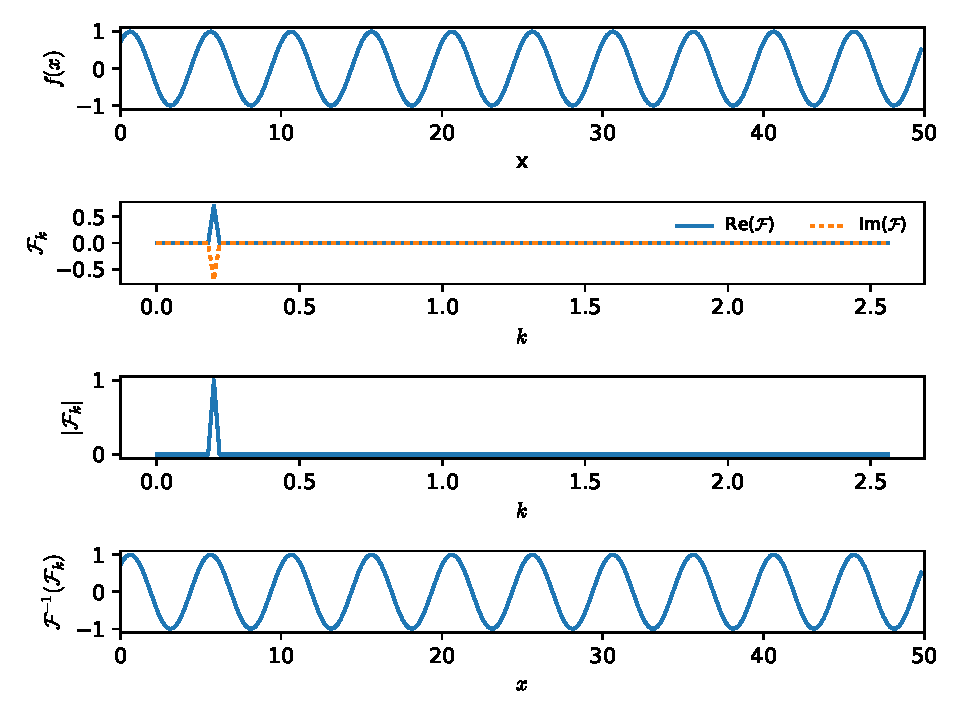
\includegraphics[width=\linewidth]{fft-sine-phase}
\caption[Fourier transform of $f(x) = \sin(2\pi k_0 x +
  \pi/4)$]{\label{fig:intro:fft} The Fourier transform of a sine wave
  with a phase of $\pi/4$, $f(x) = \sin(2\pi k_0 x + \pi/4)$ with $k_0
  = 0.2$.  The top shows the original function.  The second panel
  shows the real and imaginary components---we see all of the power is
  at our input wavenumber, split equally between the real and
  imaginary parts.  The third pane shows the power (the absolute value
  of the transform).  Finally, the bottom panel shows the inverse
  transform of our transform, giving us back our original function. \\
  \hydroexdoit{\href{https://github.com/zingale/hydro_examples/blob/master/basic_numerics/FFT/fft_simple_examples.py}{fft\_simple\_examples.py}}}
\end{figure}




%% \section{A Sample of Public Codes}

%% There are a large number of freely-available codes for modeling astrophysical
%% flows.
